% Created by tikzDevice version 0.12.6 on 2026-11-06 07:53:49
% !TEX encoding = UTF-8 Unicode
\documentclass[tikz,border=0pt]{standalone}\usepackage{tikz}
\usetikzlibrary{calc}
\usepackage[T1]{fontenc}
\usepackage[sc]{mathpazo}
\usepackage{amsmath}\begin{document}

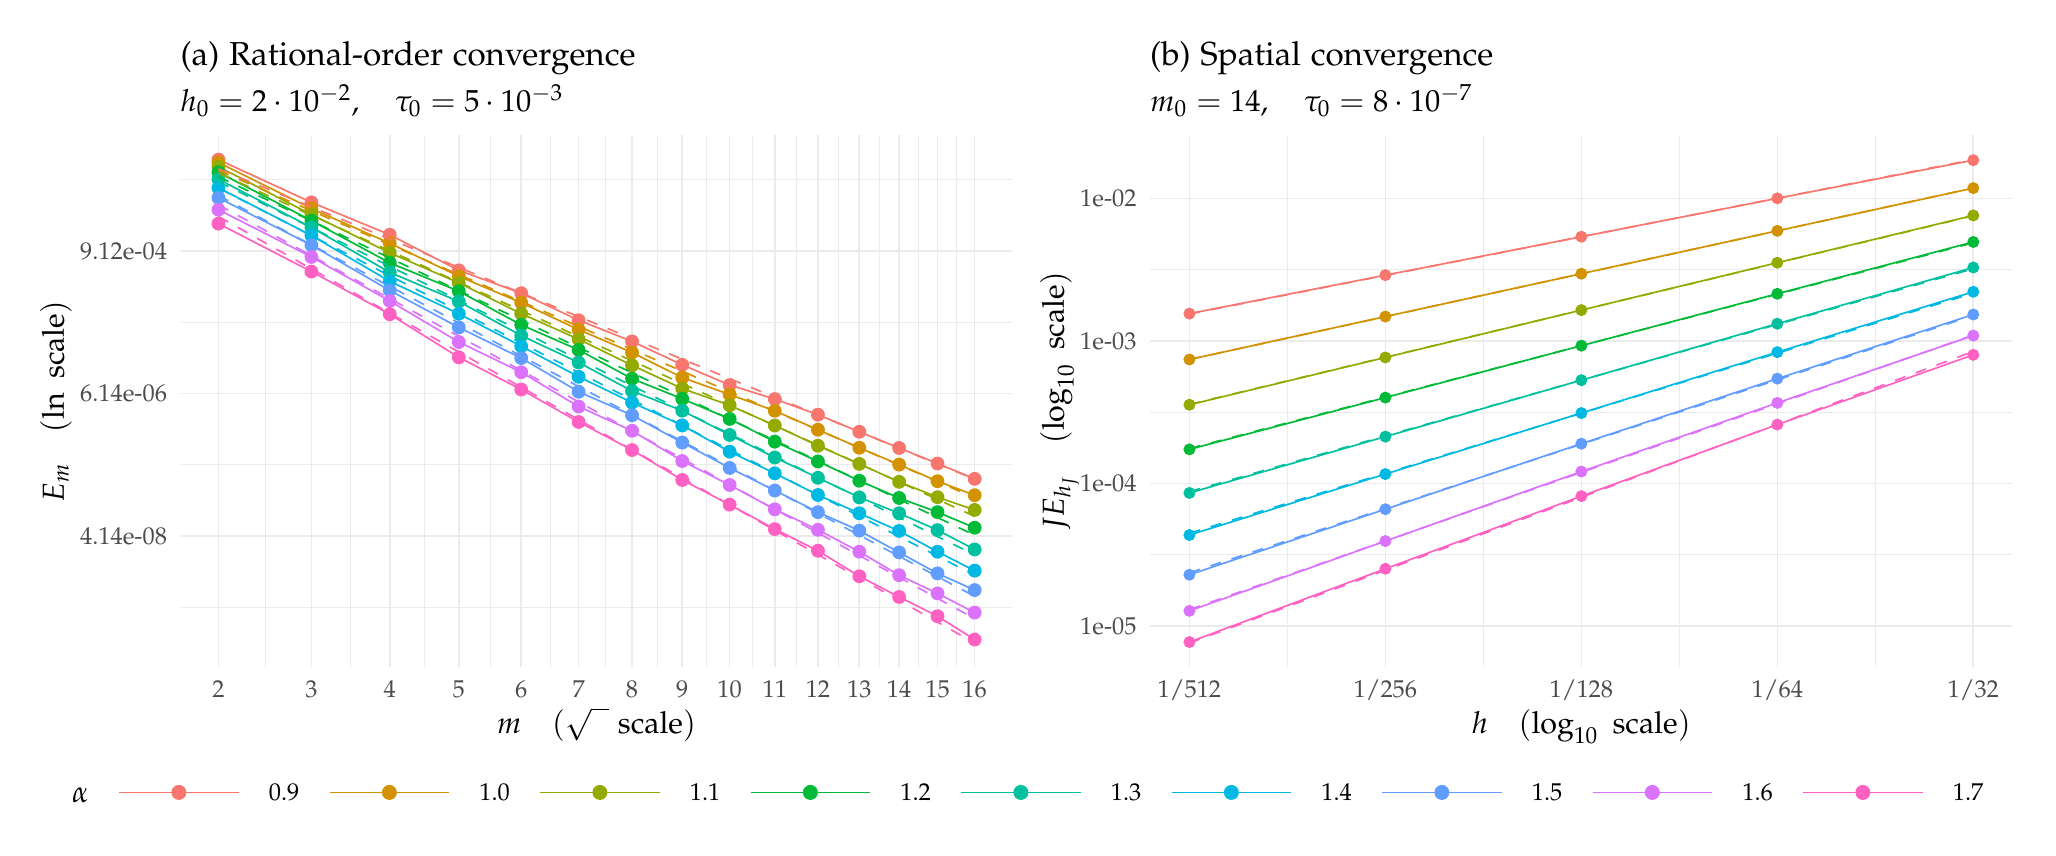
\begin{tikzpicture}[x=1pt,y=1pt]
\definecolor{fillColor}{RGB}{255,255,255}
\path[use as bounding box,fill=fillColor,fill opacity=0.00] (0,0) rectangle (722.70,289.08);
\begin{scope}
\path[clip] (  0.00, 25.45) rectangle (361.35,289.08);
\definecolor{fillColor}{RGB}{255,255,255}

\path[fill=fillColor] (  0.00, 25.45) rectangle (361.35,289.08);
\end{scope}
\begin{scope}
\path[clip] ( 55.28, 57.98) rectangle (355.85,250.13);
\definecolor{drawColor}{gray}{0.92}

\path[draw=drawColor,line width= 0.3pt,line join=round] ( 55.28, 79.71) --
	(355.85, 79.71);

\path[draw=drawColor,line width= 0.3pt,line join=round] ( 55.28,131.17) --
	(355.85,131.17);

\path[draw=drawColor,line width= 0.3pt,line join=round] ( 55.28,182.62) --
	(355.85,182.62);

\path[draw=drawColor,line width= 0.3pt,line join=round] ( 55.28,234.07) --
	(355.85,234.07);

\path[draw=drawColor,line width= 0.3pt,line join=round] ( 85.74, 57.98) --
	( 85.74,250.13);

\path[draw=drawColor,line width= 0.3pt,line join=round] (116.69, 57.98) --
	(116.69,250.13);

\path[draw=drawColor,line width= 0.3pt,line join=round] (143.32, 57.98) --
	(143.32,250.13);

\path[draw=drawColor,line width= 0.3pt,line join=round] (167.07, 57.98) --
	(167.07,250.13);

\path[draw=drawColor,line width= 0.3pt,line join=round] (188.71, 57.98) --
	(188.71,250.13);

\path[draw=drawColor,line width= 0.3pt,line join=round] (208.73, 57.98) --
	(208.73,250.13);

\path[draw=drawColor,line width= 0.3pt,line join=round] (227.45, 57.98) --
	(227.45,250.13);

\path[draw=drawColor,line width= 0.3pt,line join=round] (245.09, 57.98) --
	(245.09,250.13);

\path[draw=drawColor,line width= 0.3pt,line join=round] (261.82, 57.98) --
	(261.82,250.13);

\path[draw=drawColor,line width= 0.3pt,line join=round] (277.77, 57.98) --
	(277.77,250.13);

\path[draw=drawColor,line width= 0.3pt,line join=round] (293.03, 57.98) --
	(293.03,250.13);

\path[draw=drawColor,line width= 0.3pt,line join=round] (307.70, 57.98) --
	(307.70,250.13);

\path[draw=drawColor,line width= 0.3pt,line join=round] (321.83, 57.98) --
	(321.83,250.13);

\path[draw=drawColor,line width= 0.3pt,line join=round] (335.48, 57.98) --
	(335.48,250.13);

\path[draw=drawColor,line width= 0.6pt,line join=round] ( 55.28,105.44) --
	(355.85,105.44);

\path[draw=drawColor,line width= 0.6pt,line join=round] ( 55.28,156.89) --
	(355.85,156.89);

\path[draw=drawColor,line width= 0.6pt,line join=round] ( 55.28,208.35) --
	(355.85,208.35);

\path[draw=drawColor,line width= 0.6pt,line join=round] ( 68.94, 57.98) --
	( 68.94,250.13);

\path[draw=drawColor,line width= 0.6pt,line join=round] (102.53, 57.98) --
	(102.53,250.13);

\path[draw=drawColor,line width= 0.6pt,line join=round] (130.84, 57.98) --
	(130.84,250.13);

\path[draw=drawColor,line width= 0.6pt,line join=round] (155.79, 57.98) --
	(155.79,250.13);

\path[draw=drawColor,line width= 0.6pt,line join=round] (178.34, 57.98) --
	(178.34,250.13);

\path[draw=drawColor,line width= 0.6pt,line join=round] (199.08, 57.98) --
	(199.08,250.13);

\path[draw=drawColor,line width= 0.6pt,line join=round] (218.39, 57.98) --
	(218.39,250.13);

\path[draw=drawColor,line width= 0.6pt,line join=round] (236.52, 57.98) --
	(236.52,250.13);

\path[draw=drawColor,line width= 0.6pt,line join=round] (253.66, 57.98) --
	(253.66,250.13);

\path[draw=drawColor,line width= 0.6pt,line join=round] (269.97, 57.98) --
	(269.97,250.13);

\path[draw=drawColor,line width= 0.6pt,line join=round] (285.56, 57.98) --
	(285.56,250.13);

\path[draw=drawColor,line width= 0.6pt,line join=round] (300.51, 57.98) --
	(300.51,250.13);

\path[draw=drawColor,line width= 0.6pt,line join=round] (314.89, 57.98) --
	(314.89,250.13);

\path[draw=drawColor,line width= 0.6pt,line join=round] (328.77, 57.98) --
	(328.77,250.13);

\path[draw=drawColor,line width= 0.6pt,line join=round] (342.19, 57.98) --
	(342.19,250.13);
\definecolor{drawColor}{RGB}{248,118,109}

\path[draw=drawColor,line width= 0.6pt,line join=round] ( 68.94,241.40) --
	(102.53,225.95) --
	(130.84,214.25) --
	(155.79,201.38) --
	(178.34,193.13) --
	(199.08,183.37) --
	(218.39,175.71) --
	(236.52,167.25) --
	(253.66,159.94) --
	(269.97,154.87) --
	(285.56,149.23) --
	(300.51,143.05) --
	(314.89,137.20) --
	(328.77,131.58) --
	(342.19,126.04);
\definecolor{drawColor}{RGB}{211,146,0}

\path[draw=drawColor,line width= 0.6pt,line join=round] ( 68.94,240.36) --
	(102.53,223.70) --
	(130.84,211.19) --
	(155.79,199.25) --
	(178.34,189.69) --
	(199.08,179.96) --
	(218.39,171.70) --
	(236.52,162.65) --
	(253.66,156.52) --
	(269.97,150.62) --
	(285.56,143.79) --
	(300.51,137.28) --
	(314.89,131.19) --
	(328.77,125.19) --
	(342.19,120.13);
\definecolor{drawColor}{RGB}{147,170,0}

\path[draw=drawColor,line width= 0.6pt,line join=round] ( 68.94,238.85) --
	(102.53,221.54) --
	(130.84,207.72) --
	(155.79,196.85) --
	(178.34,185.75) --
	(199.08,176.50) --
	(218.39,167.06) --
	(236.52,158.68) --
	(253.66,152.62) --
	(269.97,145.32) --
	(285.56,138.01) --
	(300.51,131.45) --
	(314.89,124.96) --
	(328.77,119.42) --
	(342.19,114.81);
\definecolor{drawColor}{RGB}{0,186,56}

\path[draw=drawColor,line width= 0.6pt,line join=round] ( 68.94,236.83) --
	(102.53,219.35) --
	(130.84,204.11) --
	(155.79,193.85) --
	(178.34,181.69) --
	(199.08,172.63) --
	(218.39,162.23) --
	(236.52,154.97) --
	(253.66,147.70) --
	(269.97,139.48) --
	(285.56,132.33) --
	(300.51,125.37) --
	(314.89,119.13) --
	(328.77,114.01) --
	(342.19,108.38);
\definecolor{drawColor}{RGB}{0,193,159}

\path[draw=drawColor,line width= 0.6pt,line join=round] ( 68.94,234.29) --
	(102.53,216.91) --
	(130.84,200.66) --
	(155.79,190.13) --
	(178.34,177.81) --
	(199.08,168.10) --
	(218.39,157.78) --
	(236.52,150.67) --
	(253.66,141.91) --
	(269.97,133.76) --
	(285.56,126.43) --
	(300.51,119.35) --
	(314.89,113.61) --
	(328.77,107.53) --
	(342.19,100.53);
\definecolor{drawColor}{RGB}{0,185,227}

\path[draw=drawColor,line width= 0.6pt,line join=round] ( 68.94,231.21) --
	(102.53,214.01) --
	(130.84,197.42) --
	(155.79,185.72) --
	(178.34,173.97) --
	(199.08,162.95) --
	(218.39,153.62) --
	(236.52,145.36) --
	(253.66,135.86) --
	(269.97,128.04) --
	(285.56,120.21) --
	(300.51,113.61) --
	(314.89,107.22) --
	(328.77, 99.71) --
	(342.19, 92.87);
\definecolor{drawColor}{RGB}{97,156,255}

\path[draw=drawColor,line width= 0.6pt,line join=round] ( 68.94,227.57) --
	(102.53,210.49) --
	(130.84,194.12) --
	(155.79,180.76) --
	(178.34,169.69) --
	(199.08,157.53) --
	(218.39,149.02) --
	(236.52,139.16) --
	(253.66,129.98) --
	(269.97,121.81) --
	(285.56,114.02) --
	(300.51,107.33) --
	(314.89, 99.47) --
	(328.77, 91.88) --
	(342.19, 85.86);
\definecolor{drawColor}{RGB}{219,114,251}

\path[draw=drawColor,line width= 0.6pt,line join=round] ( 68.94,223.30) --
	(102.53,206.22) --
	(130.84,190.31) --
	(155.79,175.49) --
	(178.34,164.57) --
	(199.08,152.18) --
	(218.39,143.40) --
	(236.52,132.49) --
	(253.66,123.83) --
	(269.97,115.04) --
	(285.56,107.63) --
	(300.51, 99.72) --
	(314.89, 91.24) --
	(328.77, 84.65) --
	(342.19, 77.72);
\definecolor{drawColor}{RGB}{255,97,195}

\path[draw=drawColor,line width= 0.6pt,line join=round] ( 68.94,218.27) --
	(102.53,200.96) --
	(130.84,185.52) --
	(155.79,169.96) --
	(178.34,158.32) --
	(199.08,146.59) --
	(218.39,136.46) --
	(236.52,125.65) --
	(253.66,116.73) --
	(269.97,107.88) --
	(285.56,100.07) --
	(300.51, 90.85) --
	(314.89, 83.37) --
	(328.77, 76.41) --
	(342.19, 67.97);
\definecolor{fillColor}{RGB}{248,118,109}

\path[fill=fillColor] ( 68.94,241.40) circle (  2.50);

\path[fill=fillColor] (102.53,225.95) circle (  2.50);

\path[fill=fillColor] (130.84,214.25) circle (  2.50);

\path[fill=fillColor] (155.79,201.38) circle (  2.50);

\path[fill=fillColor] (178.34,193.13) circle (  2.50);

\path[fill=fillColor] (199.08,183.37) circle (  2.50);

\path[fill=fillColor] (218.39,175.71) circle (  2.50);

\path[fill=fillColor] (236.52,167.25) circle (  2.50);

\path[fill=fillColor] (253.66,159.94) circle (  2.50);

\path[fill=fillColor] (269.97,154.87) circle (  2.50);

\path[fill=fillColor] (285.56,149.23) circle (  2.50);

\path[fill=fillColor] (300.51,143.05) circle (  2.50);

\path[fill=fillColor] (314.89,137.20) circle (  2.50);

\path[fill=fillColor] (328.77,131.58) circle (  2.50);

\path[fill=fillColor] (342.19,126.04) circle (  2.50);
\definecolor{fillColor}{RGB}{211,146,0}

\path[fill=fillColor] ( 68.94,240.36) circle (  2.50);

\path[fill=fillColor] (102.53,223.70) circle (  2.50);

\path[fill=fillColor] (130.84,211.19) circle (  2.50);

\path[fill=fillColor] (155.79,199.25) circle (  2.50);

\path[fill=fillColor] (178.34,189.69) circle (  2.50);

\path[fill=fillColor] (199.08,179.96) circle (  2.50);

\path[fill=fillColor] (218.39,171.70) circle (  2.50);

\path[fill=fillColor] (236.52,162.65) circle (  2.50);

\path[fill=fillColor] (253.66,156.52) circle (  2.50);

\path[fill=fillColor] (269.97,150.62) circle (  2.50);

\path[fill=fillColor] (285.56,143.79) circle (  2.50);

\path[fill=fillColor] (300.51,137.28) circle (  2.50);

\path[fill=fillColor] (314.89,131.19) circle (  2.50);

\path[fill=fillColor] (328.77,125.19) circle (  2.50);

\path[fill=fillColor] (342.19,120.13) circle (  2.50);
\definecolor{fillColor}{RGB}{147,170,0}

\path[fill=fillColor] ( 68.94,238.85) circle (  2.50);

\path[fill=fillColor] (102.53,221.54) circle (  2.50);

\path[fill=fillColor] (130.84,207.72) circle (  2.50);

\path[fill=fillColor] (155.79,196.85) circle (  2.50);

\path[fill=fillColor] (178.34,185.75) circle (  2.50);

\path[fill=fillColor] (199.08,176.50) circle (  2.50);

\path[fill=fillColor] (218.39,167.06) circle (  2.50);

\path[fill=fillColor] (236.52,158.68) circle (  2.50);

\path[fill=fillColor] (253.66,152.62) circle (  2.50);

\path[fill=fillColor] (269.97,145.32) circle (  2.50);

\path[fill=fillColor] (285.56,138.01) circle (  2.50);

\path[fill=fillColor] (300.51,131.45) circle (  2.50);

\path[fill=fillColor] (314.89,124.96) circle (  2.50);

\path[fill=fillColor] (328.77,119.42) circle (  2.50);

\path[fill=fillColor] (342.19,114.81) circle (  2.50);
\definecolor{fillColor}{RGB}{0,186,56}

\path[fill=fillColor] ( 68.94,236.83) circle (  2.50);

\path[fill=fillColor] (102.53,219.35) circle (  2.50);

\path[fill=fillColor] (130.84,204.11) circle (  2.50);

\path[fill=fillColor] (155.79,193.85) circle (  2.50);

\path[fill=fillColor] (178.34,181.69) circle (  2.50);

\path[fill=fillColor] (199.08,172.63) circle (  2.50);

\path[fill=fillColor] (218.39,162.23) circle (  2.50);

\path[fill=fillColor] (236.52,154.97) circle (  2.50);

\path[fill=fillColor] (253.66,147.70) circle (  2.50);

\path[fill=fillColor] (269.97,139.48) circle (  2.50);

\path[fill=fillColor] (285.56,132.33) circle (  2.50);

\path[fill=fillColor] (300.51,125.37) circle (  2.50);

\path[fill=fillColor] (314.89,119.13) circle (  2.50);

\path[fill=fillColor] (328.77,114.01) circle (  2.50);

\path[fill=fillColor] (342.19,108.38) circle (  2.50);
\definecolor{fillColor}{RGB}{0,193,159}

\path[fill=fillColor] ( 68.94,234.29) circle (  2.50);

\path[fill=fillColor] (102.53,216.91) circle (  2.50);

\path[fill=fillColor] (130.84,200.66) circle (  2.50);

\path[fill=fillColor] (155.79,190.13) circle (  2.50);

\path[fill=fillColor] (178.34,177.81) circle (  2.50);

\path[fill=fillColor] (199.08,168.10) circle (  2.50);

\path[fill=fillColor] (218.39,157.78) circle (  2.50);

\path[fill=fillColor] (236.52,150.67) circle (  2.50);

\path[fill=fillColor] (253.66,141.91) circle (  2.50);

\path[fill=fillColor] (269.97,133.76) circle (  2.50);

\path[fill=fillColor] (285.56,126.43) circle (  2.50);

\path[fill=fillColor] (300.51,119.35) circle (  2.50);

\path[fill=fillColor] (314.89,113.61) circle (  2.50);

\path[fill=fillColor] (328.77,107.53) circle (  2.50);

\path[fill=fillColor] (342.19,100.53) circle (  2.50);
\definecolor{fillColor}{RGB}{0,185,227}

\path[fill=fillColor] ( 68.94,231.21) circle (  2.50);

\path[fill=fillColor] (102.53,214.01) circle (  2.50);

\path[fill=fillColor] (130.84,197.42) circle (  2.50);

\path[fill=fillColor] (155.79,185.72) circle (  2.50);

\path[fill=fillColor] (178.34,173.97) circle (  2.50);

\path[fill=fillColor] (199.08,162.95) circle (  2.50);

\path[fill=fillColor] (218.39,153.62) circle (  2.50);

\path[fill=fillColor] (236.52,145.36) circle (  2.50);

\path[fill=fillColor] (253.66,135.86) circle (  2.50);

\path[fill=fillColor] (269.97,128.04) circle (  2.50);

\path[fill=fillColor] (285.56,120.21) circle (  2.50);

\path[fill=fillColor] (300.51,113.61) circle (  2.50);

\path[fill=fillColor] (314.89,107.22) circle (  2.50);

\path[fill=fillColor] (328.77, 99.71) circle (  2.50);

\path[fill=fillColor] (342.19, 92.87) circle (  2.50);
\definecolor{fillColor}{RGB}{97,156,255}

\path[fill=fillColor] ( 68.94,227.57) circle (  2.50);

\path[fill=fillColor] (102.53,210.49) circle (  2.50);

\path[fill=fillColor] (130.84,194.12) circle (  2.50);

\path[fill=fillColor] (155.79,180.76) circle (  2.50);

\path[fill=fillColor] (178.34,169.69) circle (  2.50);

\path[fill=fillColor] (199.08,157.53) circle (  2.50);

\path[fill=fillColor] (218.39,149.02) circle (  2.50);

\path[fill=fillColor] (236.52,139.16) circle (  2.50);

\path[fill=fillColor] (253.66,129.98) circle (  2.50);

\path[fill=fillColor] (269.97,121.81) circle (  2.50);

\path[fill=fillColor] (285.56,114.02) circle (  2.50);

\path[fill=fillColor] (300.51,107.33) circle (  2.50);

\path[fill=fillColor] (314.89, 99.47) circle (  2.50);

\path[fill=fillColor] (328.77, 91.88) circle (  2.50);

\path[fill=fillColor] (342.19, 85.86) circle (  2.50);
\definecolor{fillColor}{RGB}{219,114,251}

\path[fill=fillColor] ( 68.94,223.30) circle (  2.50);

\path[fill=fillColor] (102.53,206.22) circle (  2.50);

\path[fill=fillColor] (130.84,190.31) circle (  2.50);

\path[fill=fillColor] (155.79,175.49) circle (  2.50);

\path[fill=fillColor] (178.34,164.57) circle (  2.50);

\path[fill=fillColor] (199.08,152.18) circle (  2.50);

\path[fill=fillColor] (218.39,143.40) circle (  2.50);

\path[fill=fillColor] (236.52,132.49) circle (  2.50);

\path[fill=fillColor] (253.66,123.83) circle (  2.50);

\path[fill=fillColor] (269.97,115.04) circle (  2.50);

\path[fill=fillColor] (285.56,107.63) circle (  2.50);

\path[fill=fillColor] (300.51, 99.72) circle (  2.50);

\path[fill=fillColor] (314.89, 91.24) circle (  2.50);

\path[fill=fillColor] (328.77, 84.65) circle (  2.50);

\path[fill=fillColor] (342.19, 77.72) circle (  2.50);
\definecolor{fillColor}{RGB}{255,97,195}

\path[fill=fillColor] ( 68.94,218.27) circle (  2.50);

\path[fill=fillColor] (102.53,200.96) circle (  2.50);

\path[fill=fillColor] (130.84,185.52) circle (  2.50);

\path[fill=fillColor] (155.79,169.96) circle (  2.50);

\path[fill=fillColor] (178.34,158.32) circle (  2.50);

\path[fill=fillColor] (199.08,146.59) circle (  2.50);

\path[fill=fillColor] (218.39,136.46) circle (  2.50);

\path[fill=fillColor] (236.52,125.65) circle (  2.50);

\path[fill=fillColor] (253.66,116.73) circle (  2.50);

\path[fill=fillColor] (269.97,107.88) circle (  2.50);

\path[fill=fillColor] (285.56,100.07) circle (  2.50);

\path[fill=fillColor] (300.51, 90.85) circle (  2.50);

\path[fill=fillColor] (314.89, 83.37) circle (  2.50);

\path[fill=fillColor] (328.77, 76.41) circle (  2.50);

\path[fill=fillColor] (342.19, 67.97) circle (  2.50);
\definecolor{drawColor}{RGB}{248,118,109}

\path[draw=drawColor,line width= 0.6pt,dash pattern=on 4pt off 4pt ,line join=round] ( 68.94,238.08) --
	(102.53,224.29) --
	(130.84,212.67) --
	(155.79,202.43) --
	(178.34,193.18) --
	(199.08,184.66) --
	(218.39,176.74) --
	(236.52,169.30) --
	(253.66,162.26) --
	(269.97,155.56) --
	(285.56,149.17) --
	(300.51,143.03) --
	(314.89,137.13) --
	(328.77,131.43) --
	(342.19,125.92);
\definecolor{drawColor}{RGB}{211,146,0}

\path[draw=drawColor,line width= 0.6pt,dash pattern=on 4pt off 4pt ,line join=round] ( 68.94,237.45) --
	(102.53,222.92) --
	(130.84,210.67) --
	(155.79,199.87) --
	(178.34,190.12) --
	(199.08,181.14) --
	(218.39,172.79) --
	(236.52,164.95) --
	(253.66,157.53) --
	(269.97,150.47) --
	(285.56,143.73) --
	(300.51,137.26) --
	(314.89,131.04) --
	(328.77,125.03) --
	(342.19,119.23);
\definecolor{drawColor}{RGB}{147,170,0}

\path[draw=drawColor,line width= 0.6pt,dash pattern=on 4pt off 4pt ,line join=round] ( 68.94,236.52) --
	(102.53,221.28) --
	(130.84,208.43) --
	(155.79,197.11) --
	(178.34,186.87) --
	(199.08,177.46) --
	(218.39,168.70) --
	(236.52,160.48) --
	(253.66,152.69) --
	(269.97,145.29) --
	(285.56,138.22) --
	(300.51,131.44) --
	(314.89,124.91) --
	(328.77,118.61) --
	(342.19,112.52);
\definecolor{drawColor}{RGB}{0,186,56}

\path[draw=drawColor,line width= 0.6pt,dash pattern=on 4pt off 4pt ,line join=round] ( 68.94,235.20) --
	(102.53,219.28) --
	(130.84,205.86) --
	(155.79,194.04) --
	(178.34,183.35) --
	(199.08,173.52) --
	(218.39,164.37) --
	(236.52,155.78) --
	(253.66,147.65) --
	(269.97,139.92) --
	(285.56,132.53) --
	(300.51,125.45) --
	(314.89,118.63) --
	(328.77,112.06) --
	(342.19,105.69);
\definecolor{drawColor}{RGB}{0,193,159}

\path[draw=drawColor,line width= 0.6pt,dash pattern=on 4pt off 4pt ,line join=round] ( 68.94,233.39) --
	(102.53,216.82) --
	(130.84,202.86) --
	(155.79,190.55) --
	(178.34,179.42) --
	(199.08,169.19) --
	(218.39,159.67) --
	(236.52,150.73) --
	(253.66,142.27) --
	(269.97,134.22) --
	(285.56,126.53) --
	(300.51,119.16) --
	(314.89,112.06) --
	(328.77,105.22) --
	(342.19, 98.60);
\definecolor{drawColor}{RGB}{0,185,227}

\path[draw=drawColor,line width= 0.6pt,dash pattern=on 4pt off 4pt ,line join=round] ( 68.94,231.12) --
	(102.53,213.92) --
	(130.84,199.43) --
	(155.79,186.66) --
	(178.34,175.11) --
	(199.08,164.50) --
	(218.39,154.61) --
	(236.52,145.33) --
	(253.66,136.55) --
	(269.97,128.20) --
	(285.56,120.23) --
	(300.51,112.57) --
	(314.89,105.21) --
	(328.77, 98.11) --
	(342.19, 91.23);
\definecolor{drawColor}{RGB}{97,156,255}

\path[draw=drawColor,line width= 0.6pt,dash pattern=on 4pt off 4pt ,line join=round] ( 68.94,228.40) --
	(102.53,210.60) --
	(130.84,195.60) --
	(155.79,182.38) --
	(178.34,170.43) --
	(199.08,159.44) --
	(218.39,149.21) --
	(236.52,139.60) --
	(253.66,130.52) --
	(269.97,121.87) --
	(285.56,113.61) --
	(300.51,105.69) --
	(314.89, 98.07) --
	(328.77, 90.72) --
	(342.19, 83.61);
\definecolor{drawColor}{RGB}{219,114,251}

\path[draw=drawColor,line width= 0.6pt,dash pattern=on 4pt off 4pt ,line join=round] ( 68.94,225.07) --
	(102.53,206.69) --
	(130.84,191.19) --
	(155.79,177.54) --
	(178.34,165.20) --
	(199.08,153.85) --
	(218.39,143.28) --
	(236.52,133.36) --
	(253.66,123.98) --
	(269.97,115.05) --
	(285.56,106.52) --
	(300.51, 98.34) --
	(314.89, 90.47) --
	(328.77, 82.87) --
	(342.19, 75.53);
\definecolor{drawColor}{RGB}{255,97,195}

\path[draw=drawColor,line width= 0.6pt,dash pattern=on 4pt off 4pt ,line join=round] ( 68.94,220.86) --
	(102.53,201.91) --
	(130.84,185.94) --
	(155.79,171.86) --
	(178.34,159.14) --
	(199.08,147.44) --
	(218.39,136.55) --
	(236.52,126.32) --
	(253.66,116.65) --
	(269.97,107.45) --
	(285.56, 98.66) --
	(300.51, 90.23) --
	(314.89, 82.11) --
	(328.77, 74.28) --
	(342.19, 66.71);
\end{scope}
\begin{scope}
\path[clip] (  0.00,  0.00) rectangle (722.70,289.08);
\definecolor{drawColor}{gray}{0.30}

\node[text=drawColor,anchor=base east,inner sep=0pt, outer sep=0pt, scale=  0.88] at ( 50.33,102.39) {4.14e-08};

\node[text=drawColor,anchor=base east,inner sep=0pt, outer sep=0pt, scale=  0.88] at ( 50.33,153.84) {6.14e-06};

\node[text=drawColor,anchor=base east,inner sep=0pt, outer sep=0pt, scale=  0.88] at ( 50.33,205.30) {9.12e-04};
\end{scope}
\begin{scope}
\path[clip] (  0.00,  0.00) rectangle (722.70,289.08);
\definecolor{drawColor}{gray}{0.30}

\node[text=drawColor,anchor=base,inner sep=0pt, outer sep=0pt, scale=  0.88] at ( 68.94, 46.93) {2};

\node[text=drawColor,anchor=base,inner sep=0pt, outer sep=0pt, scale=  0.88] at (102.53, 46.93) {3};

\node[text=drawColor,anchor=base,inner sep=0pt, outer sep=0pt, scale=  0.88] at (130.84, 46.93) {4};

\node[text=drawColor,anchor=base,inner sep=0pt, outer sep=0pt, scale=  0.88] at (155.79, 46.93) {5};

\node[text=drawColor,anchor=base,inner sep=0pt, outer sep=0pt, scale=  0.88] at (178.34, 46.93) {6};

\node[text=drawColor,anchor=base,inner sep=0pt, outer sep=0pt, scale=  0.88] at (199.08, 46.93) {7};

\node[text=drawColor,anchor=base,inner sep=0pt, outer sep=0pt, scale=  0.88] at (218.39, 46.93) {8};

\node[text=drawColor,anchor=base,inner sep=0pt, outer sep=0pt, scale=  0.88] at (236.52, 46.93) {9};

\node[text=drawColor,anchor=base,inner sep=0pt, outer sep=0pt, scale=  0.88] at (253.66, 46.93) {10};

\node[text=drawColor,anchor=base,inner sep=0pt, outer sep=0pt, scale=  0.88] at (269.97, 46.93) {11};

\node[text=drawColor,anchor=base,inner sep=0pt, outer sep=0pt, scale=  0.88] at (285.56, 46.93) {12};

\node[text=drawColor,anchor=base,inner sep=0pt, outer sep=0pt, scale=  0.88] at (300.51, 46.93) {13};

\node[text=drawColor,anchor=base,inner sep=0pt, outer sep=0pt, scale=  0.88] at (314.89, 46.93) {14};

\node[text=drawColor,anchor=base,inner sep=0pt, outer sep=0pt, scale=  0.88] at (328.77, 46.93) {15};

\node[text=drawColor,anchor=base,inner sep=0pt, outer sep=0pt, scale=  0.88] at (342.19, 46.93) {16};
\end{scope}
\begin{scope}
\path[clip] (  0.00,  0.00) rectangle (722.70,289.08);
\definecolor{drawColor}{RGB}{0,0,0}

\node[text=drawColor,anchor=base,inner sep=0pt, outer sep=0pt, scale=  1.10] at (205.57, 34.07) {$m\quad(\sqrt{\phantom{x}}\mbox{ scale})$};
\end{scope}
\begin{scope}
\path[clip] (  0.00,  0.00) rectangle (722.70,289.08);
\definecolor{drawColor}{RGB}{0,0,0}

\node[text=drawColor,rotate= 90.00,anchor=base,inner sep=0pt, outer sep=0pt, scale=  1.10] at ( 13.12,154.06) {$E_m\quad(\ln\mbox{ scale})$};
\end{scope}
\begin{scope}
\path[clip] (  0.00,  0.00) rectangle (722.70,289.08);
\definecolor{drawColor}{RGB}{0,0,0}

\node[text=drawColor,anchor=base west,inner sep=0pt, outer sep=0pt, scale=  1.10] at ( 55.28,258.75) {$h_0=2\cdot10^{-2},\quad\tau_0=5\cdot10^{-3}$};
\end{scope}
\begin{scope}
\path[clip] (  0.00,  0.00) rectangle (722.70,289.08);
\definecolor{drawColor}{RGB}{0,0,0}

\node[text=drawColor,anchor=base west,inner sep=0pt, outer sep=0pt, scale=  1.20] at ( 55.28,275.26) {(a) Rational-order convergence};
\end{scope}
\begin{scope}
\path[clip] (361.35, 25.45) rectangle (722.70,289.08);
\definecolor{fillColor}{RGB}{255,255,255}

\path[fill=fillColor] (361.35, 25.45) rectangle (722.70,289.08);
\end{scope}
\begin{scope}
\path[clip] (405.63, 57.98) rectangle (717.20,250.13);
\definecolor{drawColor}{gray}{0.92}

\path[draw=drawColor,line width= 0.3pt,line join=round] (405.63, 98.67) --
	(717.20, 98.67);

\path[draw=drawColor,line width= 0.3pt,line join=round] (405.63,150.15) --
	(717.20,150.15);

\path[draw=drawColor,line width= 0.3pt,line join=round] (405.63,201.62) --
	(717.20,201.62);

\path[draw=drawColor,line width= 0.3pt,line join=round] (667.63, 57.98) --
	(667.63,250.13);

\path[draw=drawColor,line width= 0.3pt,line join=round] (596.82, 57.98) --
	(596.82,250.13);

\path[draw=drawColor,line width= 0.3pt,line join=round] (526.01, 57.98) --
	(526.01,250.13);

\path[draw=drawColor,line width= 0.3pt,line join=round] (455.20, 57.98) --
	(455.20,250.13);

\path[draw=drawColor,line width= 0.6pt,line join=round] (405.63, 72.94) --
	(717.20, 72.94);

\path[draw=drawColor,line width= 0.6pt,line join=round] (405.63,124.41) --
	(717.20,124.41);

\path[draw=drawColor,line width= 0.6pt,line join=round] (405.63,175.89) --
	(717.20,175.89);

\path[draw=drawColor,line width= 0.6pt,line join=round] (405.63,227.36) --
	(717.20,227.36);

\path[draw=drawColor,line width= 0.6pt,line join=round] (703.04, 57.98) --
	(703.04,250.13);

\path[draw=drawColor,line width= 0.6pt,line join=round] (632.23, 57.98) --
	(632.23,250.13);

\path[draw=drawColor,line width= 0.6pt,line join=round] (561.42, 57.98) --
	(561.42,250.13);

\path[draw=drawColor,line width= 0.6pt,line join=round] (490.60, 57.98) --
	(490.60,250.13);

\path[draw=drawColor,line width= 0.6pt,line join=round] (419.79, 57.98) --
	(419.79,250.13);
\definecolor{drawColor}{RGB}{248,118,109}

\path[draw=drawColor,line width= 0.6pt,dash pattern=on 4pt off 4pt ,line join=round] (419.79,185.62) --
	(490.60,199.56) --
	(561.42,213.51) --
	(632.23,227.45) --
	(703.04,241.40);
\definecolor{drawColor}{RGB}{211,146,0}

\path[draw=drawColor,line width= 0.6pt,dash pattern=on 4pt off 4pt ,line join=round] (419.79,169.17) --
	(490.60,184.66) --
	(561.42,200.16) --
	(632.23,215.65) --
	(703.04,231.15);
\definecolor{drawColor}{RGB}{147,170,0}

\path[draw=drawColor,line width= 0.6pt,dash pattern=on 4pt off 4pt ,line join=round] (419.79,152.93) --
	(490.60,169.98) --
	(561.42,187.02) --
	(632.23,204.07) --
	(703.04,221.11);
\definecolor{drawColor}{RGB}{0,186,56}

\path[draw=drawColor,line width= 0.6pt,dash pattern=on 4pt off 4pt ,line join=round] (419.79,136.98) --
	(490.60,155.57) --
	(561.42,174.17) --
	(632.23,192.76) --
	(703.04,211.35);
\definecolor{drawColor}{RGB}{0,193,159}

\path[draw=drawColor,line width= 0.6pt,dash pattern=on 4pt off 4pt ,line join=round] (419.79,121.41) --
	(490.60,141.55) --
	(561.42,161.70) --
	(632.23,181.84) --
	(703.04,201.98);
\definecolor{drawColor}{RGB}{0,185,227}

\path[draw=drawColor,line width= 0.6pt,dash pattern=on 4pt off 4pt ,line join=round] (419.79,106.38) --
	(490.60,128.07) --
	(561.42,149.77) --
	(632.23,171.46) --
	(703.04,193.15);
\definecolor{drawColor}{RGB}{97,156,255}

\path[draw=drawColor,line width= 0.6pt,dash pattern=on 4pt off 4pt ,line join=round] (419.79, 92.10) --
	(490.60,115.34) --
	(561.42,138.58) --
	(632.23,161.82) --
	(703.04,185.07);
\definecolor{drawColor}{RGB}{219,114,251}

\path[draw=drawColor,line width= 0.6pt,dash pattern=on 4pt off 4pt ,line join=round] (419.79, 78.80) --
	(490.60,103.60) --
	(561.42,128.39) --
	(632.23,153.18) --
	(703.04,177.97);
\definecolor{drawColor}{RGB}{255,97,195}

\path[draw=drawColor,line width= 0.6pt,dash pattern=on 4pt off 4pt ,line join=round] (419.79, 66.71) --
	(490.60, 93.05) --
	(561.42,119.40) --
	(632.23,145.74) --
	(703.04,172.08);
\definecolor{drawColor}{RGB}{248,118,109}

\path[draw=drawColor,line width= 0.6pt,line join=round] (419.79,185.75) --
	(490.60,199.65) --
	(561.42,213.54) --
	(632.23,227.40) --
	(703.04,241.19);
\definecolor{drawColor}{RGB}{211,146,0}

\path[draw=drawColor,line width= 0.6pt,line join=round] (419.79,169.18) --
	(490.60,184.68) --
	(561.42,200.17) --
	(632.23,215.66) --
	(703.04,231.10);
\definecolor{drawColor}{RGB}{147,170,0}

\path[draw=drawColor,line width= 0.6pt,line join=round] (419.79,152.81) --
	(490.60,169.91) --
	(561.42,187.02) --
	(632.23,204.14) --
	(703.04,221.23);
\definecolor{drawColor}{RGB}{0,186,56}

\path[draw=drawColor,line width= 0.6pt,line join=round] (419.79,136.70) --
	(490.60,155.41) --
	(561.42,174.16) --
	(632.23,192.92) --
	(703.04,211.64);
\definecolor{drawColor}{RGB}{0,193,159}

\path[draw=drawColor,line width= 0.6pt,line join=round] (419.79,120.95) --
	(490.60,141.30) --
	(561.42,161.70) --
	(632.23,182.11) --
	(703.04,202.41);
\definecolor{drawColor}{RGB}{0,185,227}

\path[draw=drawColor,line width= 0.6pt,line join=round] (419.79,105.75) --
	(490.60,127.77) --
	(561.42,149.82) --
	(632.23,171.83) --
	(703.04,193.64);
\definecolor{drawColor}{RGB}{97,156,255}

\path[draw=drawColor,line width= 0.6pt,line join=round] (419.79, 91.39) --
	(490.60,115.08) --
	(561.42,138.74) --
	(632.23,162.25) --
	(703.04,185.43);
\definecolor{drawColor}{RGB}{219,114,251}

\path[draw=drawColor,line width= 0.6pt,line join=round] (419.79, 78.34) --
	(490.60,103.57) --
	(561.42,128.68) --
	(632.23,153.50) --
	(703.04,177.82);
\definecolor{drawColor}{RGB}{255,97,195}

\path[draw=drawColor,line width= 0.6pt,line join=round] (419.79, 67.07) --
	(490.60, 93.55) --
	(561.42,119.81) --
	(632.23,145.65) --
	(703.04,170.86);
\definecolor{drawColor}{RGB}{248,118,109}
\definecolor{fillColor}{RGB}{248,118,109}

\path[draw=drawColor,line width= 0.4pt,line join=round,line cap=round,fill=fillColor] (703.04,241.19) circle (  1.96);

\path[draw=drawColor,line width= 0.4pt,line join=round,line cap=round,fill=fillColor] (632.23,227.40) circle (  1.96);

\path[draw=drawColor,line width= 0.4pt,line join=round,line cap=round,fill=fillColor] (561.42,213.54) circle (  1.96);

\path[draw=drawColor,line width= 0.4pt,line join=round,line cap=round,fill=fillColor] (490.60,199.65) circle (  1.96);

\path[draw=drawColor,line width= 0.4pt,line join=round,line cap=round,fill=fillColor] (419.79,185.75) circle (  1.96);
\definecolor{drawColor}{RGB}{211,146,0}
\definecolor{fillColor}{RGB}{211,146,0}

\path[draw=drawColor,line width= 0.4pt,line join=round,line cap=round,fill=fillColor] (703.04,231.10) circle (  1.96);

\path[draw=drawColor,line width= 0.4pt,line join=round,line cap=round,fill=fillColor] (632.23,215.66) circle (  1.96);

\path[draw=drawColor,line width= 0.4pt,line join=round,line cap=round,fill=fillColor] (561.42,200.17) circle (  1.96);

\path[draw=drawColor,line width= 0.4pt,line join=round,line cap=round,fill=fillColor] (490.60,184.68) circle (  1.96);

\path[draw=drawColor,line width= 0.4pt,line join=round,line cap=round,fill=fillColor] (419.79,169.18) circle (  1.96);
\definecolor{drawColor}{RGB}{147,170,0}
\definecolor{fillColor}{RGB}{147,170,0}

\path[draw=drawColor,line width= 0.4pt,line join=round,line cap=round,fill=fillColor] (703.04,221.23) circle (  1.96);

\path[draw=drawColor,line width= 0.4pt,line join=round,line cap=round,fill=fillColor] (632.23,204.14) circle (  1.96);

\path[draw=drawColor,line width= 0.4pt,line join=round,line cap=round,fill=fillColor] (561.42,187.02) circle (  1.96);

\path[draw=drawColor,line width= 0.4pt,line join=round,line cap=round,fill=fillColor] (490.60,169.91) circle (  1.96);

\path[draw=drawColor,line width= 0.4pt,line join=round,line cap=round,fill=fillColor] (419.79,152.81) circle (  1.96);
\definecolor{drawColor}{RGB}{0,186,56}
\definecolor{fillColor}{RGB}{0,186,56}

\path[draw=drawColor,line width= 0.4pt,line join=round,line cap=round,fill=fillColor] (703.04,211.64) circle (  1.96);

\path[draw=drawColor,line width= 0.4pt,line join=round,line cap=round,fill=fillColor] (632.23,192.92) circle (  1.96);

\path[draw=drawColor,line width= 0.4pt,line join=round,line cap=round,fill=fillColor] (561.42,174.16) circle (  1.96);

\path[draw=drawColor,line width= 0.4pt,line join=round,line cap=round,fill=fillColor] (490.60,155.41) circle (  1.96);

\path[draw=drawColor,line width= 0.4pt,line join=round,line cap=round,fill=fillColor] (419.79,136.70) circle (  1.96);
\definecolor{drawColor}{RGB}{0,193,159}
\definecolor{fillColor}{RGB}{0,193,159}

\path[draw=drawColor,line width= 0.4pt,line join=round,line cap=round,fill=fillColor] (703.04,202.41) circle (  1.96);

\path[draw=drawColor,line width= 0.4pt,line join=round,line cap=round,fill=fillColor] (632.23,182.11) circle (  1.96);

\path[draw=drawColor,line width= 0.4pt,line join=round,line cap=round,fill=fillColor] (561.42,161.70) circle (  1.96);

\path[draw=drawColor,line width= 0.4pt,line join=round,line cap=round,fill=fillColor] (490.60,141.30) circle (  1.96);

\path[draw=drawColor,line width= 0.4pt,line join=round,line cap=round,fill=fillColor] (419.79,120.95) circle (  1.96);
\definecolor{drawColor}{RGB}{0,185,227}
\definecolor{fillColor}{RGB}{0,185,227}

\path[draw=drawColor,line width= 0.4pt,line join=round,line cap=round,fill=fillColor] (703.04,193.64) circle (  1.96);

\path[draw=drawColor,line width= 0.4pt,line join=round,line cap=round,fill=fillColor] (632.23,171.83) circle (  1.96);

\path[draw=drawColor,line width= 0.4pt,line join=round,line cap=round,fill=fillColor] (561.42,149.82) circle (  1.96);

\path[draw=drawColor,line width= 0.4pt,line join=round,line cap=round,fill=fillColor] (490.60,127.77) circle (  1.96);

\path[draw=drawColor,line width= 0.4pt,line join=round,line cap=round,fill=fillColor] (419.79,105.75) circle (  1.96);
\definecolor{drawColor}{RGB}{97,156,255}
\definecolor{fillColor}{RGB}{97,156,255}

\path[draw=drawColor,line width= 0.4pt,line join=round,line cap=round,fill=fillColor] (703.04,185.43) circle (  1.96);

\path[draw=drawColor,line width= 0.4pt,line join=round,line cap=round,fill=fillColor] (632.23,162.25) circle (  1.96);

\path[draw=drawColor,line width= 0.4pt,line join=round,line cap=round,fill=fillColor] (561.42,138.74) circle (  1.96);

\path[draw=drawColor,line width= 0.4pt,line join=round,line cap=round,fill=fillColor] (490.60,115.08) circle (  1.96);

\path[draw=drawColor,line width= 0.4pt,line join=round,line cap=round,fill=fillColor] (419.79, 91.39) circle (  1.96);
\definecolor{drawColor}{RGB}{219,114,251}
\definecolor{fillColor}{RGB}{219,114,251}

\path[draw=drawColor,line width= 0.4pt,line join=round,line cap=round,fill=fillColor] (703.04,177.82) circle (  1.96);

\path[draw=drawColor,line width= 0.4pt,line join=round,line cap=round,fill=fillColor] (632.23,153.50) circle (  1.96);

\path[draw=drawColor,line width= 0.4pt,line join=round,line cap=round,fill=fillColor] (561.42,128.68) circle (  1.96);

\path[draw=drawColor,line width= 0.4pt,line join=round,line cap=round,fill=fillColor] (490.60,103.57) circle (  1.96);

\path[draw=drawColor,line width= 0.4pt,line join=round,line cap=round,fill=fillColor] (419.79, 78.34) circle (  1.96);
\definecolor{drawColor}{RGB}{255,97,195}
\definecolor{fillColor}{RGB}{255,97,195}

\path[draw=drawColor,line width= 0.4pt,line join=round,line cap=round,fill=fillColor] (703.04,170.86) circle (  1.96);

\path[draw=drawColor,line width= 0.4pt,line join=round,line cap=round,fill=fillColor] (632.23,145.65) circle (  1.96);

\path[draw=drawColor,line width= 0.4pt,line join=round,line cap=round,fill=fillColor] (561.42,119.81) circle (  1.96);

\path[draw=drawColor,line width= 0.4pt,line join=round,line cap=round,fill=fillColor] (490.60, 93.55) circle (  1.96);

\path[draw=drawColor,line width= 0.4pt,line join=round,line cap=round,fill=fillColor] (419.79, 67.07) circle (  1.96);
\end{scope}
\begin{scope}
\path[clip] (  0.00,  0.00) rectangle (722.70,289.08);
\definecolor{drawColor}{gray}{0.30}

\node[text=drawColor,anchor=base east,inner sep=0pt, outer sep=0pt, scale=  0.88] at (400.68, 69.89) {1e-05};

\node[text=drawColor,anchor=base east,inner sep=0pt, outer sep=0pt, scale=  0.88] at (400.68,121.36) {1e-04};

\node[text=drawColor,anchor=base east,inner sep=0pt, outer sep=0pt, scale=  0.88] at (400.68,172.84) {1e-03};

\node[text=drawColor,anchor=base east,inner sep=0pt, outer sep=0pt, scale=  0.88] at (400.68,224.31) {1e-02};
\end{scope}
\begin{scope}
\path[clip] (  0.00,  0.00) rectangle (722.70,289.08);
\definecolor{drawColor}{gray}{0.30}

\node[text=drawColor,anchor=base,inner sep=0pt, outer sep=0pt, scale=  0.88] at (703.04, 46.93) {1/32};

\node[text=drawColor,anchor=base,inner sep=0pt, outer sep=0pt, scale=  0.88] at (632.23, 46.93) {1/64};

\node[text=drawColor,anchor=base,inner sep=0pt, outer sep=0pt, scale=  0.88] at (561.42, 46.93) {1/128};

\node[text=drawColor,anchor=base,inner sep=0pt, outer sep=0pt, scale=  0.88] at (490.60, 46.93) {1/256};

\node[text=drawColor,anchor=base,inner sep=0pt, outer sep=0pt, scale=  0.88] at (419.79, 46.93) {1/512};
\end{scope}
\begin{scope}
\path[clip] (  0.00,  0.00) rectangle (722.70,289.08);
\definecolor{drawColor}{RGB}{0,0,0}

\node[text=drawColor,anchor=base,inner sep=0pt, outer sep=0pt, scale=  1.10] at (561.42, 34.07) {$h\quad(\log_{10}\mbox{ scale})$};
\end{scope}
\begin{scope}
\path[clip] (  0.00,  0.00) rectangle (722.70,289.08);
\definecolor{drawColor}{RGB}{0,0,0}

\node[text=drawColor,rotate= 90.00,anchor=base,inner sep=0pt, outer sep=0pt, scale=  1.10] at (374.47,154.06) {$JE_{h_J}\quad(\log_{10}\mbox{ scale})$};
\end{scope}
\begin{scope}
\path[clip] (  0.00,  0.00) rectangle (722.70,289.08);
\definecolor{drawColor}{RGB}{0,0,0}

\node[text=drawColor,anchor=base west,inner sep=0pt, outer sep=0pt, scale=  1.10] at (405.63,258.75) {$m_0=14,\quad\tau_0=8\cdot10^{-7}$};
\end{scope}
\begin{scope}
\path[clip] (  0.00,  0.00) rectangle (722.70,289.08);
\definecolor{drawColor}{RGB}{0,0,0}

\node[text=drawColor,anchor=base west,inner sep=0pt, outer sep=0pt, scale=  1.20] at (405.63,275.26) {(b) Spatial convergence};
\end{scope}
\begin{scope}
\path[clip] (  0.00,  0.00) rectangle (722.70,289.08);
\definecolor{drawColor}{RGB}{0,0,0}

\node[text=drawColor,anchor=base west,inner sep=0pt, outer sep=0pt, scale=  1.10] at ( 16.04,  8.92) {$\alpha$};
\end{scope}
\begin{scope}
\path[clip] (  0.00,  0.00) rectangle (722.70,289.08);
\definecolor{drawColor}{RGB}{248,118,109}

\path[draw=drawColor,line width= 0.6pt,line join=round] ( 33.03, 12.73) -- ( 76.27, 12.73);
\end{scope}
\begin{scope}
\path[clip] (  0.00,  0.00) rectangle (722.70,289.08);
\definecolor{drawColor}{RGB}{248,118,109}
\definecolor{fillColor}{RGB}{248,118,109}

\path[draw=drawColor,line width= 0.4pt,line join=round,line cap=round,fill=fillColor] ( 54.65, 12.73) circle (  2.50);
\end{scope}
\begin{scope}
\path[clip] (  0.00,  0.00) rectangle (722.70,289.08);
\definecolor{drawColor}{RGB}{248,118,109}

\path[draw=drawColor,line width= 0.6pt,dash pattern=on 4pt off 4pt ,line join=round] ( 33.03, 12.73) -- ( 76.27, 12.73);
\end{scope}
\begin{scope}
\path[clip] (  0.00,  0.00) rectangle (722.70,289.08);
\definecolor{drawColor}{RGB}{211,146,0}

\path[draw=drawColor,line width= 0.6pt,line join=round] (109.09, 12.73) -- (152.33, 12.73);
\end{scope}
\begin{scope}
\path[clip] (  0.00,  0.00) rectangle (722.70,289.08);
\definecolor{drawColor}{RGB}{211,146,0}
\definecolor{fillColor}{RGB}{211,146,0}

\path[draw=drawColor,line width= 0.4pt,line join=round,line cap=round,fill=fillColor] (130.71, 12.73) circle (  2.50);
\end{scope}
\begin{scope}
\path[clip] (  0.00,  0.00) rectangle (722.70,289.08);
\definecolor{drawColor}{RGB}{211,146,0}

\path[draw=drawColor,line width= 0.6pt,dash pattern=on 4pt off 4pt ,line join=round] (109.09, 12.73) -- (152.33, 12.73);
\end{scope}
\begin{scope}
\path[clip] (  0.00,  0.00) rectangle (722.70,289.08);
\definecolor{drawColor}{RGB}{147,170,0}

\path[draw=drawColor,line width= 0.6pt,line join=round] (185.15, 12.73) -- (228.39, 12.73);
\end{scope}
\begin{scope}
\path[clip] (  0.00,  0.00) rectangle (722.70,289.08);
\definecolor{drawColor}{RGB}{147,170,0}
\definecolor{fillColor}{RGB}{147,170,0}

\path[draw=drawColor,line width= 0.4pt,line join=round,line cap=round,fill=fillColor] (206.77, 12.73) circle (  2.50);
\end{scope}
\begin{scope}
\path[clip] (  0.00,  0.00) rectangle (722.70,289.08);
\definecolor{drawColor}{RGB}{147,170,0}

\path[draw=drawColor,line width= 0.6pt,dash pattern=on 4pt off 4pt ,line join=round] (185.15, 12.73) -- (228.39, 12.73);
\end{scope}
\begin{scope}
\path[clip] (  0.00,  0.00) rectangle (722.70,289.08);
\definecolor{drawColor}{RGB}{0,186,56}

\path[draw=drawColor,line width= 0.6pt,line join=round] (261.21, 12.73) -- (304.46, 12.73);
\end{scope}
\begin{scope}
\path[clip] (  0.00,  0.00) rectangle (722.70,289.08);
\definecolor{drawColor}{RGB}{0,186,56}
\definecolor{fillColor}{RGB}{0,186,56}

\path[draw=drawColor,line width= 0.4pt,line join=round,line cap=round,fill=fillColor] (282.83, 12.73) circle (  2.50);
\end{scope}
\begin{scope}
\path[clip] (  0.00,  0.00) rectangle (722.70,289.08);
\definecolor{drawColor}{RGB}{0,186,56}

\path[draw=drawColor,line width= 0.6pt,dash pattern=on 4pt off 4pt ,line join=round] (261.21, 12.73) -- (304.46, 12.73);
\end{scope}
\begin{scope}
\path[clip] (  0.00,  0.00) rectangle (722.70,289.08);
\definecolor{drawColor}{RGB}{0,193,159}

\path[draw=drawColor,line width= 0.6pt,line join=round] (337.27, 12.73) -- (380.52, 12.73);
\end{scope}
\begin{scope}
\path[clip] (  0.00,  0.00) rectangle (722.70,289.08);
\definecolor{drawColor}{RGB}{0,193,159}
\definecolor{fillColor}{RGB}{0,193,159}

\path[draw=drawColor,line width= 0.4pt,line join=round,line cap=round,fill=fillColor] (358.89, 12.73) circle (  2.50);
\end{scope}
\begin{scope}
\path[clip] (  0.00,  0.00) rectangle (722.70,289.08);
\definecolor{drawColor}{RGB}{0,193,159}

\path[draw=drawColor,line width= 0.6pt,dash pattern=on 4pt off 4pt ,line join=round] (337.27, 12.73) -- (380.52, 12.73);
\end{scope}
\begin{scope}
\path[clip] (  0.00,  0.00) rectangle (722.70,289.08);
\definecolor{drawColor}{RGB}{0,185,227}

\path[draw=drawColor,line width= 0.6pt,line join=round] (413.33, 12.73) -- (456.58, 12.73);
\end{scope}
\begin{scope}
\path[clip] (  0.00,  0.00) rectangle (722.70,289.08);
\definecolor{drawColor}{RGB}{0,185,227}
\definecolor{fillColor}{RGB}{0,185,227}

\path[draw=drawColor,line width= 0.4pt,line join=round,line cap=round,fill=fillColor] (434.95, 12.73) circle (  2.50);
\end{scope}
\begin{scope}
\path[clip] (  0.00,  0.00) rectangle (722.70,289.08);
\definecolor{drawColor}{RGB}{0,185,227}

\path[draw=drawColor,line width= 0.6pt,dash pattern=on 4pt off 4pt ,line join=round] (413.33, 12.73) -- (456.58, 12.73);
\end{scope}
\begin{scope}
\path[clip] (  0.00,  0.00) rectangle (722.70,289.08);
\definecolor{drawColor}{RGB}{97,156,255}

\path[draw=drawColor,line width= 0.6pt,line join=round] (489.39, 12.73) -- (532.64, 12.73);
\end{scope}
\begin{scope}
\path[clip] (  0.00,  0.00) rectangle (722.70,289.08);
\definecolor{drawColor}{RGB}{97,156,255}
\definecolor{fillColor}{RGB}{97,156,255}

\path[draw=drawColor,line width= 0.4pt,line join=round,line cap=round,fill=fillColor] (511.01, 12.73) circle (  2.50);
\end{scope}
\begin{scope}
\path[clip] (  0.00,  0.00) rectangle (722.70,289.08);
\definecolor{drawColor}{RGB}{97,156,255}

\path[draw=drawColor,line width= 0.6pt,dash pattern=on 4pt off 4pt ,line join=round] (489.39, 12.73) -- (532.64, 12.73);
\end{scope}
\begin{scope}
\path[clip] (  0.00,  0.00) rectangle (722.70,289.08);
\definecolor{drawColor}{RGB}{219,114,251}

\path[draw=drawColor,line width= 0.6pt,line join=round] (565.45, 12.73) -- (608.70, 12.73);
\end{scope}
\begin{scope}
\path[clip] (  0.00,  0.00) rectangle (722.70,289.08);
\definecolor{drawColor}{RGB}{219,114,251}
\definecolor{fillColor}{RGB}{219,114,251}

\path[draw=drawColor,line width= 0.4pt,line join=round,line cap=round,fill=fillColor] (587.07, 12.73) circle (  2.50);
\end{scope}
\begin{scope}
\path[clip] (  0.00,  0.00) rectangle (722.70,289.08);
\definecolor{drawColor}{RGB}{219,114,251}

\path[draw=drawColor,line width= 0.6pt,dash pattern=on 4pt off 4pt ,line join=round] (565.45, 12.73) -- (608.70, 12.73);
\end{scope}
\begin{scope}
\path[clip] (  0.00,  0.00) rectangle (722.70,289.08);
\definecolor{drawColor}{RGB}{255,97,195}

\path[draw=drawColor,line width= 0.6pt,line join=round] (641.51, 12.73) -- (684.76, 12.73);
\end{scope}
\begin{scope}
\path[clip] (  0.00,  0.00) rectangle (722.70,289.08);
\definecolor{drawColor}{RGB}{255,97,195}
\definecolor{fillColor}{RGB}{255,97,195}

\path[draw=drawColor,line width= 0.4pt,line join=round,line cap=round,fill=fillColor] (663.13, 12.73) circle (  2.50);
\end{scope}
\begin{scope}
\path[clip] (  0.00,  0.00) rectangle (722.70,289.08);
\definecolor{drawColor}{RGB}{255,97,195}

\path[draw=drawColor,line width= 0.6pt,dash pattern=on 4pt off 4pt ,line join=round] (641.51, 12.73) -- (684.76, 12.73);
\end{scope}
\begin{scope}
\path[clip] (  0.00,  0.00) rectangle (722.70,289.08);
\definecolor{drawColor}{RGB}{0,0,0}

\node[text=drawColor,anchor=base west,inner sep=0pt, outer sep=0pt, scale=  0.88] at ( 87.18,  9.68) {$0.9$};
\end{scope}
\begin{scope}
\path[clip] (  0.00,  0.00) rectangle (722.70,289.08);
\definecolor{drawColor}{RGB}{0,0,0}

\node[text=drawColor,anchor=base west,inner sep=0pt, outer sep=0pt, scale=  0.88] at (163.24,  9.68) {$1.0$};
\end{scope}
\begin{scope}
\path[clip] (  0.00,  0.00) rectangle (722.70,289.08);
\definecolor{drawColor}{RGB}{0,0,0}

\node[text=drawColor,anchor=base west,inner sep=0pt, outer sep=0pt, scale=  0.88] at (239.30,  9.68) {$1.1$};
\end{scope}
\begin{scope}
\path[clip] (  0.00,  0.00) rectangle (722.70,289.08);
\definecolor{drawColor}{RGB}{0,0,0}

\node[text=drawColor,anchor=base west,inner sep=0pt, outer sep=0pt, scale=  0.88] at (315.36,  9.68) {$1.2$};
\end{scope}
\begin{scope}
\path[clip] (  0.00,  0.00) rectangle (722.70,289.08);
\definecolor{drawColor}{RGB}{0,0,0}

\node[text=drawColor,anchor=base west,inner sep=0pt, outer sep=0pt, scale=  0.88] at (391.42,  9.68) {$1.3$};
\end{scope}
\begin{scope}
\path[clip] (  0.00,  0.00) rectangle (722.70,289.08);
\definecolor{drawColor}{RGB}{0,0,0}

\node[text=drawColor,anchor=base west,inner sep=0pt, outer sep=0pt, scale=  0.88] at (467.48,  9.68) {$1.4$};
\end{scope}
\begin{scope}
\path[clip] (  0.00,  0.00) rectangle (722.70,289.08);
\definecolor{drawColor}{RGB}{0,0,0}

\node[text=drawColor,anchor=base west,inner sep=0pt, outer sep=0pt, scale=  0.88] at (543.54,  9.68) {$1.5$};
\end{scope}
\begin{scope}
\path[clip] (  0.00,  0.00) rectangle (722.70,289.08);
\definecolor{drawColor}{RGB}{0,0,0}

\node[text=drawColor,anchor=base west,inner sep=0pt, outer sep=0pt, scale=  0.88] at (619.60,  9.68) {$1.6$};
\end{scope}
\begin{scope}
\path[clip] (  0.00,  0.00) rectangle (722.70,289.08);
\definecolor{drawColor}{RGB}{0,0,0}

\node[text=drawColor,anchor=base west,inner sep=0pt, outer sep=0pt, scale=  0.88] at (695.66,  9.68) {$1.7$};
\end{scope}
\end{tikzpicture}

\end{document}
